% *********************************************************************
% © 2021–2024 Jeremy Sylvestre
%
% Permission is granted to copy, distribute and/or modify this document
% under the terms of the GNU Free Documentation License, Version 1.3 or
% any later version published by the Free Software Foundation; with no
% Invariant Sections, no Front-Cover Texts, and no Back-Cover Texts. A
% copy of the license is included in the appendix entitled “GNU Free
% Documentation License” that appears in the output document of this
% PreTeXt source code. All trademarks™ are the registered® marks of
% their respective owners.
%
% *********************************************************************

\newcommand*{\xmin}{-1}
\newcommand*{\xmax}{10.05}
\newcommand*{\ymin}{-0.25}
\newcommand*{\ymax}{2.5}

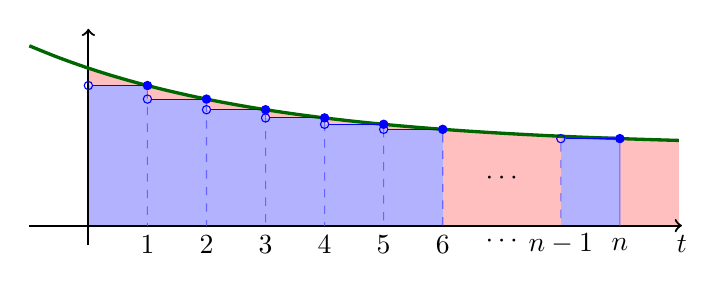
\begin{tikzpicture}
[
	closedpt/.style={circle,draw,fill,inner sep=0pt,minimum size=3pt},
	openpt/.style={circle,draw,inner sep=0pt,minimum size=3pt},
	xscale=0.75
]

	% graph fill
	\fill[red!25!white]
	  plot[domain=0:10,smooth] (\x,{exp(-\x/4) + 1})
	  -- (10,0) -- (0,0) -- (0,2);

	% rectangle fills
	\fill[blue!30!white] (0,1.779) rectangle (1,0);
	\fill[blue!30!white] (1,1.607) rectangle (2,0);
	\fill[blue!30!white] (2,1.472) rectangle (3,0);
	\fill[blue!30!white] (3,1.368) rectangle (4,0);
	\fill[blue!30!white] (4,1.287) rectangle (5,0);
	\fill[blue!30!white] (5,1.223) rectangle (6,0);
	\fill[blue!30!white] (8,1.135) rectangle (9,0);

	% axes
	\draw[->,thick] (\xmin,0) -- (\xmax,0) node[below] {$t$};
	\draw[->,thick] (0,\ymin) -- (0,\ymax);

	% label axes
	\foreach \x in {1,2,...,6} {
		\node[below] at (\x,0) {$\x$};
	}
	\node at (7,-0.2) {$\cdots$};
	\node at (7,0.6) {$\cdots$};
	\node at (8,-0.23) {$n - 1$};
	\node at (9,-0.24) {$n$};

	% continuous graph
	\draw[green!40!black,very thick,domain=-1:10,smooth] plot (\x,{exp(-\x/4) + 1});

	% levels and dividers
	\node[blue,openpt] at (0,1.779) (start) {};
	\node[blue,closedpt] at (1,1.779) (stop) {};
	\draw[blue,thin] (start.east) -- (stop.west);
	\draw[blue!60!white,dashed] (stop.south) -- (1,0);
	%
	\node[blue,openpt] at (1,1.607) (start) {};
	\node[blue,closedpt] at (2,1.607) (stop) {};
	\draw[blue,thin] (start.east) -- (stop.west);
	\draw[blue!60!white,dashed] (stop.south) -- (2,0);
	%
	\node[blue,openpt] at (2,1.472) (start) {};
	\node[blue,closedpt] at (3,1.472) (stop) {};
	\draw[blue,thin] (start.east) -- (stop.west);
	\draw[blue!60!white,dashed] (stop.south) -- (3,0);
	%
	\node[blue,openpt] at (3,1.368) (start) {};
	\node[blue,closedpt] at (4,1.368) (stop) {};
	\draw[blue,thin] (start.east) -- (stop.west);
	\draw[blue!60!white,dashed] (stop.south) -- (4,0);
	%
	\node[blue,openpt] at (4,1.287) (start) {};
	\node[blue,closedpt] at (5,1.287) (stop) {};
	\draw[blue,thin] (start.east) -- (stop.west);
	\draw[blue!60!white,dashed] (stop.south) -- (5,0);
	%
	\node[blue,openpt] at (5,1.223) (start) {};
	\node[blue,closedpt] at (6,1.223) (stop) {};
	\draw[blue,thin] (start.east) -- (stop.west);
	\draw[blue!60!white,dashed] (stop.south) -- (6,0);
	%
	\node[blue,openpt] at (8,1.105) (start) {};
	\node[blue,closedpt] at (9,1.105) (stop) {};
	\draw[blue,thin] (start.east) -- (stop.west);
	\draw[blue!60!white,dashed] (start.south) -- (8,0);
	\draw[blue!60!white] (stop.south) -- (9,0);
	%

\end{tikzpicture}
